\chapter{How Balance Leads to Productivity}

This chapter follows a School of Hard Knocks entrepreneurship lecture curated by LazyingArt LLC. The argument begins with a hard constraint, not a slogan: a day has only twenty-four hours. From there the speaker moves carefully through definition, exception, risk, and method. Balance is not presented as a perfect daily symmetry. It is a practical system for protecting mental health, preventing burnout, and preserving the energy that lets productive work continue.

\section{The Twenty-Four-Hour Constraint}

We begin where the lecture begins: with the size of the day. There are only twenty-four hours in which responsibilities, work, self-care, friends, and family can all make their claims. In the simplest bookkeeping form,

\begin{equation}
T_{\mathrm{day}} = 24\ \mathrm{hours}.
\end{equation}

This immediately turns ``balance'' into an allocation problem. If we try to put everything into the day without making choices, the arithmetic will not close. The speaker's working definition is direct: balance is making time for the things we have to do and also for the things we want to do.

A cautious reconstruction of that idea is

\begin{equation}
T_{\mathrm{day}}
=
T_{\mathrm{work}}
+
T_{\mathrm{responsibilities}}
+
T_{\mathrm{self}}
+
T_{\mathrm{family}}
+
T_{\mathrm{friends}}
+
T_{\mathrm{recovery}}.
\end{equation}

The equation is not a measured formula. It is a way of making the spoken point explicit: the day is finite, so every protected activity must be given a place inside the same finite total.

\subsection{Question \& Answer}

\paragraph{Question.}
If the day has only twenty-four hours, how do we handle responsibilities while still making time for ourselves, friends, and family?

\paragraph{Answer.}
We first stop treating balance as a vague ideal. Balance begins as a design problem: some time must go to obligations, and some time must be deliberately reserved for the rest of life. The point is not that every category receives equal time. The point is that the important categories are not left to chance.

\section{The Exception: Necessary Imbalance}

The speaker immediately qualifies the definition. This is important. Balance is not a rule that every single day can obey. There are seasons in which imbalance is real, necessary, and sometimes chosen.

For an entrepreneur working on a project that may change a life, the workday can sometimes become

\begin{equation}
T_{\mathrm{work}} \approx 16\ \mathrm{hours}.
\end{equation}

Those are not balanced days. The lecture also gives the newborn-parent example: the parent is not really making the schedule; the baby is. These examples prevent the chapter from becoming naive. We do not condemn every local imbalance. We ask whether imbalance has become the permanent operating system.

The speaker then narrows the target to the ordinary majority of life, the part where habits and systems can be installed:

\begin{equation}
0.80 \leq f_{\mathrm{ordinary}} \leq 0.85.
\end{equation}

Here \(f_{\mathrm{ordinary}}\) is not a statistic from a study. It is the speaker's estimate of the portion of life where balance can realistically be designed. Exceptional periods exist, but the rest of life should not be surrendered to accident.

\section{Why Balance Matters}

The lecture then pivots from definition to motive: why does balance matter? The first answer is mental health. The speaker does not begin with productivity tricks. He begins with the condition of the person doing the work.

When life is busy, it is easy to keep moving without asking whether the current pattern is working. The lecture's diagnostic is simple: pause and ask what is causing stress, and ask what is being prioritized.

\subsection{Question \& Answer}

\paragraph{Question.}
How do we know whether work-life balance has become unhealthy?

\paragraph{Answer.}
We inspect the state we are actually in. The speaker's test is not complicated: what is stressing me out, and what am I prioritizing right now? We can write the diagnostic state as

\begin{equation}
X_{\mathrm{life}}
=
\bigl(
S_{\mathrm{stress}},
P_{\mathrm{priority}},
D_{\mathrm{direction}}
\bigr).
\end{equation}

Here \(S_{\mathrm{stress}}\) stands for present stressors, \(P_{\mathrm{priority}}\) for what is actually receiving attention, and \(D_{\mathrm{direction}}\) for the direction life and work are taking. The notation is only a compact bookkeeping device. The real move is reflective: before we optimize the schedule, we ask whether the schedule is carrying us somewhere we still want to go.

\section{Burnout As Lost Capacity}

The second reason balance matters is burnout. The speaker defines burnout as the point where we no longer have the strength or desire to continue working on what we are working on. He describes the experience as detachment, lack of imagination, lack of creativity, and the absence of any desire to work.

For entrepreneurship, this is not merely a private feeling. It damages the system's productive capacity. Let \(C\) denote practical working capacity: the ability to think, create, decide, and continue. The lecture's mechanism can be summarized as

\begin{equation}
\mathrm{lack\ of\ balance}
\longrightarrow
\mathrm{burnout}
\longrightarrow
C \downarrow .
\end{equation}

This is not a clinical model of burnout. It is a practical model of entrepreneurial capacity. If the worker or founder becomes detached and uncreative, the project loses one of its most important inputs.

\section{Motivation And Segmentation}

The third reason balance matters is motivation at work. The speaker's point is subtle enough to preserve: time away from work is not simply the opposite of productivity. If the workday is efficient and the mind is in a better state, then the rest of life can feed energy back into the next workday.

A compact reconstruction is

\begin{equation}
\mathrm{better\ mental\ state}
+
\mathrm{efficient\ work}
\longrightarrow
\mathrm{usable\ nonwork\ time}
\longrightarrow
\mathrm{renewed\ motivation}.
\end{equation}

This is where segmentation enters. Work time is work time. Family time, hobbies, games, physical activity, and passion projects are not just scraps left after exhaustion. They are parts of the system that make continued work possible.

\begin{figure}
\centering
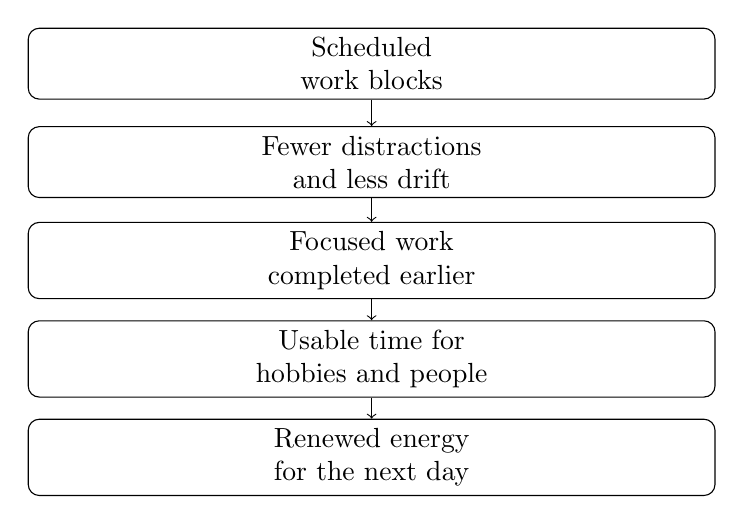
\begin{tikzpicture}
\node[draw, rounded corners, align=center, text width=0.70\linewidth] (a) at (0,0) {Scheduled\\work blocks};
\node[draw, rounded corners, align=center, text width=0.70\linewidth] (b) at (0,-1.25) {Fewer distractions\\and less drift};
\node[draw, rounded corners, align=center, text width=0.70\linewidth] (c) at (0,-2.50) {Focused work\\completed earlier};
\node[draw, rounded corners, align=center, text width=0.70\linewidth] (d) at (0,-3.75) {Usable time for\\hobbies and people};
\node[draw, rounded corners, align=center, text width=0.70\linewidth] (e) at (0,-5.00) {Renewed energy\\for the next day};
\draw[->] (a) -- (b);
\draw[->] (b) -- (c);
\draw[->] (c) -- (d);
\draw[->] (d) -- (e);
\end{tikzpicture}
\caption{A transcript-derived reconstruction of the lecture's balance mechanism. The flow is drawn vertically so it remains readable in a narrow page format.}
\end{figure}

The diagram is intentionally narrow. The lecture does not need a large life-management chart. It needs a loop: structure protects focus, focus preserves energy, and restored energy makes work sustainable.

\section{How To Become Balanced}

After explaining why balance matters, the speaker makes the practical turn: how do we actually become balanced? The answer comes in the same order as the lecture: schedule the day, prepare the workspace, keep hobbies outside work, and spend time with close people.

\subsection{Question \& Answer}

\paragraph{Question.}
How do we move from knowing that balance matters to actually building it?

\paragraph{Answer.}
We build a small operating system. The workday gets blocked. The morning is protected for deep work when distractions are lowest. The desk is arranged so focus is not repeatedly broken. Outside work, we keep activities and relationships that restore energy rather than merely filling time.

\subsection{Time Blocking}

The first practice is scheduling the day. The speaker says that mornings have become his most productive and focused period because they contain the fewest distractions. That is where he places deep work and tasks requiring the most attention.

The transcript gives concrete block sizes:

\begin{equation}
T_{\mathrm{block}}
\in
\{45\ \mathrm{min},\ 60\ \mathrm{min},\ 30\ \mathrm{min}\}.
\end{equation}

The reason for blocking is not just neatness. It controls slack. Suppose a task needs \(30\) minutes of focused effort. If we allocate \(60\) minutes, the slack is

\begin{align}
S_{60}
&=
T_{\mathrm{allocated}} - T_{\mathrm{focus}} \\
&=
60\ \mathrm{min} - 30\ \mathrm{min} \\
&=
30\ \mathrm{min}.
\end{align}

If the same task receives two hours, the slack grows:

\begin{align}
S_{120}
&=
120\ \mathrm{min} - 30\ \mathrm{min} \\
&=
90\ \mathrm{min}.
\end{align}

The speaker's warning is that this extra slack often becomes wasted time. In a compact update form,

\begin{equation}
S
=
T_{\mathrm{allocated}}
-
T_{\mathrm{focus}},
\qquad
T_{\mathrm{allocated}} \uparrow
\Rightarrow
S \uparrow
\end{equation}

when the true task requirement \(T_{\mathrm{focus}}\) stays fixed. Time blocking works by limiting the container. It gives the task enough room to be completed, but not so much room that attention dissolves.

\subsection{A Prepared Environment}

The second practice is having a clean desk and a good work environment. The point is not aesthetic. It is mechanical. If everything needed is close at hand, we do not repeatedly get up, search, reset, and re-enter the work.

Let \(I\) represent interruptions during a work block. The claim is

\begin{equation}
\mathrm{prepared\ environment}
\longrightarrow
I \downarrow
\longrightarrow
\mathrm{focus} \uparrow .
\end{equation}

A cleaner environment therefore supports the same goal as time blocking: staying in the zone long enough to finish the work efficiently.

\subsection{Hobbies Outside Work}

The third practice is having hobbies or passions outside work. The speaker gives ordinary examples: going to the gym, doing something physically active, eating dinner with friends, bowling, reading in a hammock, or playing video games. The exact activity is not the issue. The issue is whether there is some activity outside work that feels genuinely enjoyable and refreshing.

We can express the recovery mechanism as

\begin{equation}
\mathrm{enjoyable\ nonwork\ activity}
\longrightarrow
E_{\mathrm{recovery}} \uparrow
\longrightarrow
\mathrm{next\ day\ motivation} \uparrow .
\end{equation}

This keeps the chapter close to the lecture's claim. The speaker is not arguing that every evening must be productive. He is arguing that doing something genuinely enjoyed outside work can make returning to work feel fresh rather than empty.

\subsection{Family And Close Friends}

The final practice is spending time with family and close friends. The speaker frames these people as support in the darkest moments and as the first people to celebrate wins. In a business chapter, that belongs under resilience. Entrepreneurs often talk about endurance as if it were only personal toughness. Here endurance is also relational.

Close people provide a form of emotional infrastructure. They do not replace discipline, but they help the person remain steady enough to keep using discipline. A life optimized only for output can look efficient in the short run while quietly removing the support that makes long-run output possible.

\section{Summary}

The lecture unfolds as a practical theory of balance under scarcity. We start with

\begin{equation}
T_{\mathrm{day}} = 24\ \mathrm{hours},
\end{equation}

and then ask how work, responsibilities, self-care, recovery, family, and friends can live inside that finite total. The speaker allows for exceptional imbalance: entrepreneurial pushes may involve \(16\)-hour workdays, and newborn-parent schedules may not be self-directed at all. But the ordinary majority of life can still be designed.

The mechanism is sequential. Reflection identifies stress and priorities. Time blocking protects focus. A prepared environment reduces interruptions. Hobbies restore energy. Close relationships provide support. Balance, in this lecture, is not the enemy of productivity. It is one of the conditions that lets productivity continue without consuming the person who produces it.